\documentclass[12pt,a4papper]{article}


\usepackage[utf8x]{inputenc}
\usepackage[brazil]{babel}
%\usepackage{setspace} %pacote para espaçamento
\usepackage{indentfirst}
\usepackage{graphicx, wrapfig, float} %pacotes figuras/imagens
\usepackage{amsfonts, amssymb, amsmath, mathrsfs} %pacotes matémáticos
%\usepackage[top=2.5cm, bottom=3cm, left=2.5cm, right=2.5cm]{geometry} %margem
%\usepackage{algorithmic, algorithm} %algoritmos

%\onehalfspace %espacamento de um e meio
%\doublespace %espaçamento duplo

\title{NP-Completude}

\author{Breno Naodi Kusunoki \\
        \texttt{brenokusunoki@gmail.com}
        \and 
        Luiz Guilherme Castilho Martins \\
        \texttt{luizgui@gmail.com}
} 

\date{Londrina, \today}

 

\date{Londrina, \today}

\begin{document}

\maketitle
\thispagestyle{empty}
\newpage

\tableofcontents
\thispagestyle{empty}
\newpage

\section{Problemas com tempo polinomial}

Problemas com tempo polinomial ou apenas problemas \textbf{P}.
São problemas comprovadamente possíveis de serem resolvidos deterministicamente em tempo polinomial, isto é, esses problemas podem ser resolvidos no tempo $O(n^k)$ para alguma constante $k$ e $n$ o tamanho da entrada \cite{leisersonalgoritmos}.

\section{Problemas polinomiais não determinísticos}
Problemas polinomiais não determinísticos ou apenas problemas \textbf{NP} é uma classe de problemas que não se conseguiu até este momento criar algoritmos determinísticos que os resolvam em tempo satisfatório \cite{goodrichprojeto}. 

Para esse tipo de problemas utiliza-se algoritmos não determinísticos como parte da solução e cria-se mecanismos para fazer a validação da solução "encontrada". Essa validação deve ter custo polinomial para que faça sentido o uso desta abordagem. 

Podemos definir de forma mais informal que algoritmos não determinísticos são algoritmos que basicamente "escolhem" uma solução entre todas as possíveis soluções, sem nenhum critério de escolha. Essa "escolha" por sua vez tem custo $O\,(1)$ uma vez que não é realizado nenhum esforço computacional.

Pode-se acrescentar também que todos os problemas em \textbf{P} também estão em \textbf{NP}, ou seja o conjunto de problemas \textbf{P} está contido em \textbf{NP}, isso se dá pelo fato de que podemos resolver qualquer problema \textbf{P} em tempo polinomial \cite{leisersonalgoritmos}.

\begin{figure}[H]
	\centering
	\label{fig1}
	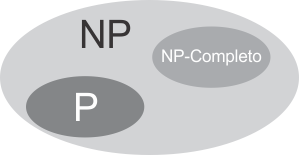
\includegraphics[scale=2]{./figuras/figProblemas.png}
	\caption{O modo como grande parte dos cientistas da computação vê os relacinamentos entre P, NP e NPC. Tanto P quanto NPC estão completamente contidas dentro de NP, e $P \cap NP-Completo = \phi$ \cite{leisersonalgoritmos}}
\end{figure}
\section{Problemas NP-Difícil}
Os problemas \textbf{NP-difícil} são problemas tão difíceis quanto qualquer outro problema \textbf{NP}. Porém só podemos afirmar que um problema é tão difícil quanto qualquer outro se ele for redutível polinomialmente a eles.

Problemas NP-Difícil são problemas que podem ser redutíveis em tempo polinomial a todos os problemas NP porém esse problema não está contido em NP.

\section{Problemas NP-Completo}
Problemas \textbf{NP-completo} são problemas que estão na classe de problemas \textbf{NP-dificil} e também estão na classe de problemas \textbf{NP}, e isso deve ser provado matematicamente assim como o \textit{Teorema de Cook} com o \textit{Problema SAT} que foi o primeiro problema comprovadamente \textbf{NP-completo}.


\section{Redutibilidade em tempo polinomial}
Redutibilidade em tempo polinomial é uma ferramenta para se reduzir um problema a outro, ou seja, utilizar um problema na solução de outro utilizando funções polinomiais denominadas algoritmos de redução.

Podemos reduzir polinomialmente um problema \textbf{A} em um problema \textbf{B} se existe uma função polinomial $f$ que transforma a entrada de \textbf{A} em entrada de \textbf{B} e também exista uma função $g$ que transforma a saída de \textbf{B} em saída de \textbf{A}. Porém existe ainda a condicional \textit{se somente se} sobre a resposta, uma vez que, se a resposta de \textbf{A} é \textit{"sim"} a resposta de \textbf{B} também deverá ser \textit{"sim"}, caso contrário a redução não existe.

\section{Transferência de cotas}
Transferência de cotas se dá quando há uma redução de um problema em outro, dessa forma existe uma transferência de cota inerente da redução.

Dada uma redução polinomial de \textbf{X} a \textbf{Y} ou seja $X \leq_P Y$ e o algoritmo de redução $f$ de tempo polinomial. Sabendo que a cota superior de \textbf{Y} é $O\,(nlgn)$ existirá uma transferência da cota superior de \textbf{Y} para a cota inferior de \textbf{X} acrescido do tempo do algoritmo de redução ou seja o a cota inferior de \textbf{X} será $O\,(nlgn\,+\,f)$


\section{Exemplos}

\subsection{O Problema da Coloração de Grafos}
Um grafo $G\:(V,E)$ pode ser "colorido" com $k$ cores?

O problema de otimização da coloração de grafos consiste em determinar o número mínimo de cores
necessárias para colorir um grafo de forma que não exista 2 vértices adjacentes com a mesma cor. 
Este número é chamado de número cromático.

\subsection{O Problema do Clique}

Um clique em um grafo G é um subconjunto C de vértices tal que, para cada $v$ e $w$ em C com $v \neq w$, ($v$,$w$) é uma aresta.
O problema recebe como entrada um grafo G e um inteiro $k$ e efetua a pergunta se há um clique em G de tamanho mínimo $k$ \cite{goodrichprojeto}.



\nocite{HOPCROFT1974}
\nocite{VIEIRA2001}
\nocite{SKIENA2010}
\nocite{NEAPOLITAN1997}
\nocite{MANBER1989}

\bibliographystyle{ieeetr}
\bibliography{bibliografia}


\end{document}
